\subsubsection{問題A01 The First Problem}

\begin{toi*}
  整数$N$が与えられるので、一辺の長さが$N$であるような正方形の面積を出力するプログラムを作成してください。
\end{toi*}

\begin{ans*}
解答は以下のようになります。
\begin{lstlisting}[caption={}]
main = print . (^2) =<< readLn
\end{lstlisting}
おっと、いきなり驚かせてしまいました。訳わからないですよね。Haskellで競プロを行うにあたって、
入出力をどうするかが最初の大きな壁となります。入出力はモナドという概念が使われており、そのモナドを
理解することがそもそも難しいからです。ここで、上記のコードを以下のように書き換えてみます。
\begin{lstlisting}[caption={}]
main = do
    n <- readLn
    print (n ^ 2)
\end{lstlisting}
何をやっているのかが見えてきましたね!\texttt{n <- readLn}で\texttt{n}に入力値を受け取っています。
そして、答えの$n^2$を\texttt{print (n \^ \ 2)}で出力します。
このように、{\bf \texttt{do}記法}(\texttt{do}構文)を用いることで命令型のプログラムに似た形で記述ができます。

ここから少し難しい話に入りますので、最初は簡単に読む程度で問題ありません。まずはGHCの対話モードを起動して\texttt{readLn}の型を問い合わせてみましょう。
\begin{verbatim}
    ghci> :t readLn
    readLn :: Read a => IO a
\end{verbatim}
\texttt{a}を型クラス\texttt{Read}の{\bf インスタンス}の型として、\texttt{readLn}の型は\texttt{IO a}となります。
言い換えると、「\texttt{readLn}は\texttt{a}を生成するIOアクションである」となります。
\begin{verbatim}
    n <- readLn
\end{verbatim}
と書くことで、IOの中身の型\texttt{a}の値を\texttt{n}に束縛することができます。すなわち、\texttt{n :: Read a => a}となります。
ではここで、エディタの拡張機能に\texttt{n}の型を教えてもらいましょう。
\begin{center}
    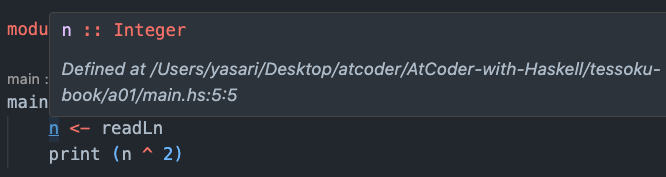
\includegraphics[width=10cm]{./src/img/a01-1.png}
\end{center}
あれ、\texttt{n :: Integer}となっています。\texttt{Read}のインスタンスは
\texttt{Int}や\texttt{Float}、\texttt{(Int, Char)}など様々な型があります。
数ある候補の中からなぜ\texttt{Integer}が選ばれたのでしょうか?それは、Haskellの{\bf 型検査器(type checker)}が賢いからです。
後ろで\texttt{n}が\texttt{n \^ \ 2}という使われ方をしているため、それなら\texttt{n}の型は\texttt{Integer}だな!と{\bf 型推論}
をしてくれます。
いやいや、ちょっと待って。俺は\texttt{n}を\texttt{Int}型として扱いたいんだ!という場合は
\begin{verbatim}
    n <- readLn :: IO Int
\end{verbatim}
と、型注釈をつけてあげましょう。初めての\texttt{AC}!嬉しいですね。
\begin{center}
    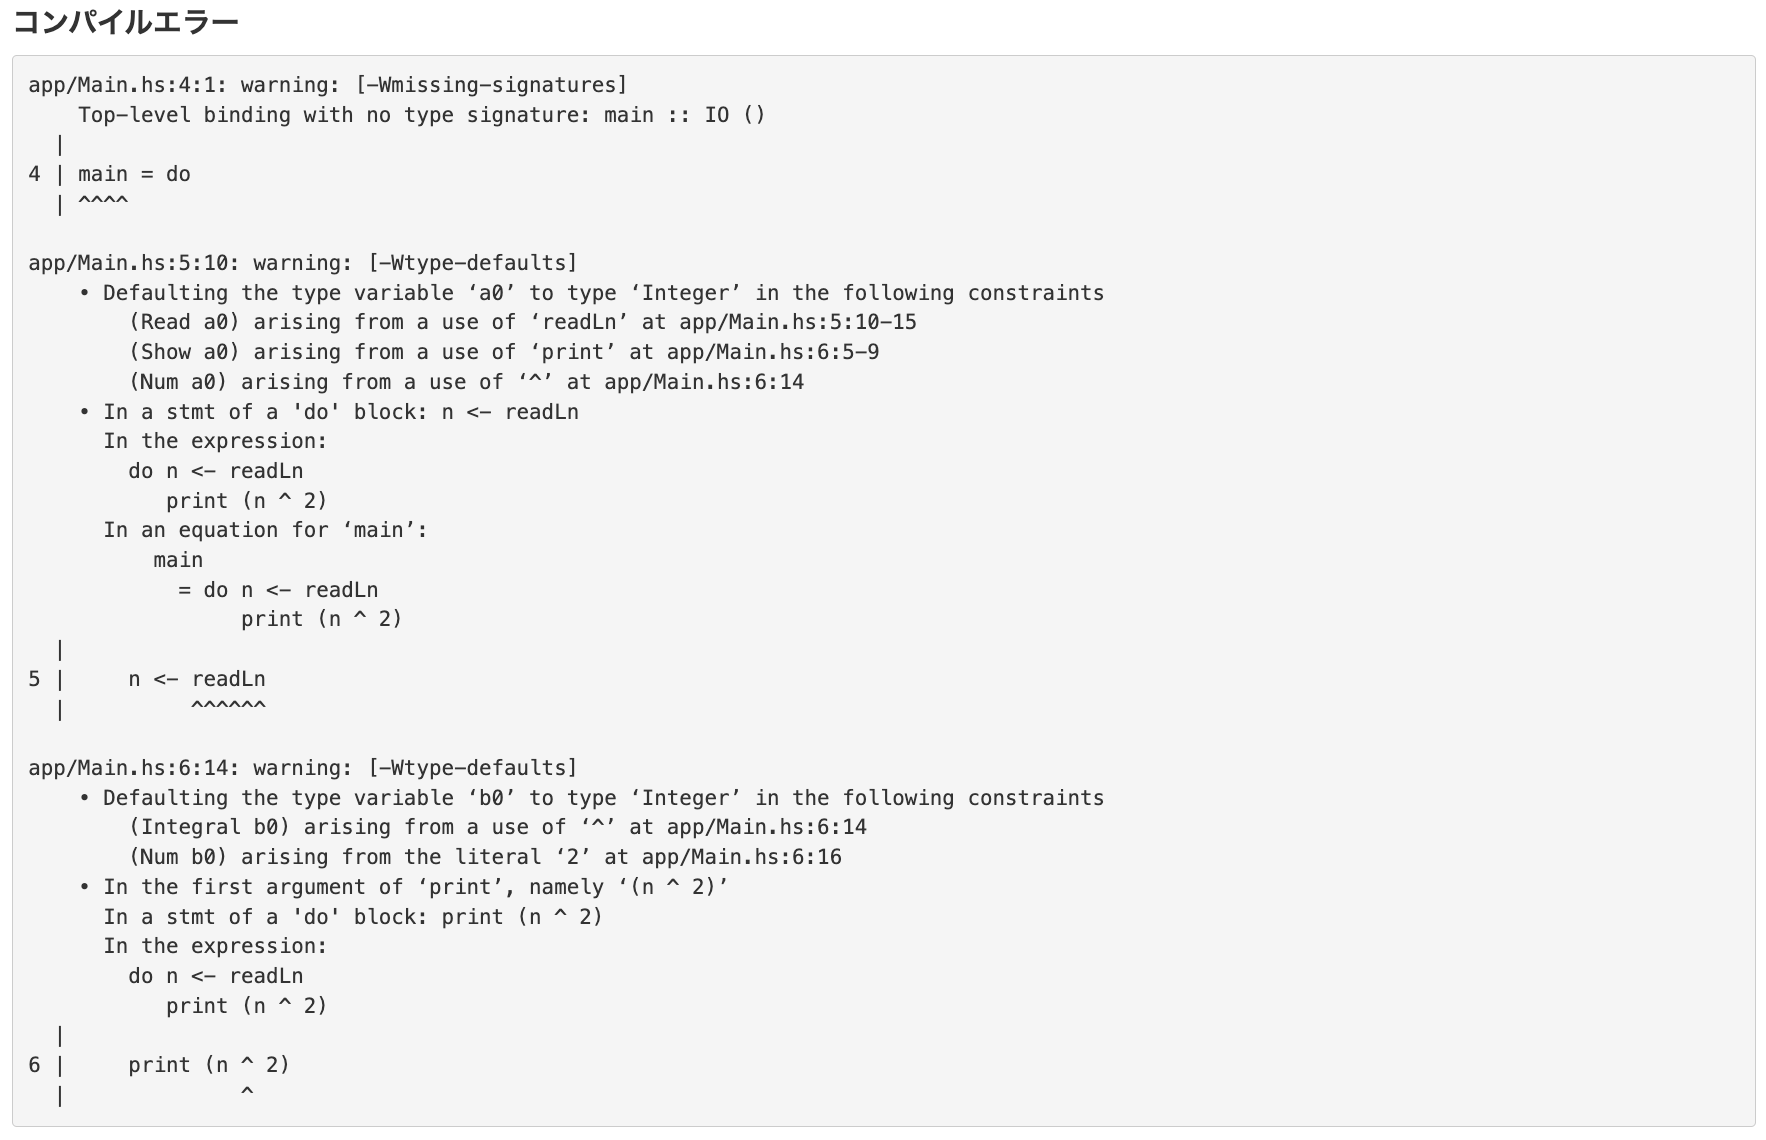
\includegraphics[width=15cm]{./src/img/a01-2.png}
\end{center}
\end{ans*}

\begin{pro*}
\noindent
\begin{lstlisting}[caption={問題A01 The First Problem},label=A01,frame={tb}]
main :: IO ()
main = do
    n <- readLn
    print (n * n)
\end{lstlisting}
\end{pro*}